%! TEX program = lualatex
\documentclass[12pt]{scrartcl}
% Packages
%\usepackage[margin=1.5in]{geometry}
\usepackage{index}
\usepackage{amsbsy} % Bold math symbols
\makeindex
%\usepackage[utf8]{inputenc}
\usepackage[T1]{fontenc}
\usepackage{tcolorbox}
\tcbuselibrary{theorems}
\tcbuselibrary{skins}
\tcbuselibrary{breakable}
\usepackage{varwidth}
\usepackage{textcomp}
\usepackage{amsmath, amssymb}
\usepackage{esint}
\usepackage{titlesec}
\usepackage{xcolor}
\usepackage{titling}
\usepackage[linktocpage]{hyperref}
\usepackage{pgfplots}
\usepackage{multicol}
\setlength{\columnsep}{2em}
\usepackage{caption}
\usepackage{amsthm}
\usepackage{import}
\usepackage{cancel}
\usepackage{caption}
\usepackage{nicematrix}
\usepackage{mathrsfs}
\usepackage{mathtools}
%\usepackage{parskip}
\usepackage{enumerate}
\usepackage{graphicx}
\usepackage[italian]{babel}
\usepackage{setspace}
\setstretch{1.2}
% To reset footnote numbering each page
\usepackage[perpage]{footmisc}
\usepackage{faktor}
\usepackage{tikz-cd}
\definecolor{mastercolor}{HTML}{0c800f}
\definecolor{nred}{HTML}{bf0040}

\usepackage{fancyhdr}
\pagestyle{fancy}

% Titles 
\title{Appunti di\\ \vspace{.3cm} Geometria e topologia differenziale}
\author{Manuel Deodato}
\date{}




\newtheoremstyle{style}% name of the style to be used
{5pt}% measure of space to leave above the theorem. E.g.: 3pt
{5pt}% measure of space to leave below the theorem. E.g.: 3pt
{\normalfont}% name of font to use in the body of the theorem
%{15pt}% measure of space to indent
{0pt}% measure of space to indent
{\noindent\sffamily\scshape\bfseries}% name of head font
{}% punctuation between head and body
{ }% space after theorem head; " " = normal interword space
{\thmname{#1}\thmnumber{ #2}{\thmnote{ (#3)}.\ }}


\theoremstyle{style}
\newtheorem{esempio}{Esempio}[section]
\newtheorem{definizione}{Definizione}[section]
\newtheorem{prop}{Proposizione}[section]
\newtheorem{teorema}{Teorema}[section]
\newtheorem{lemma}{Lemma}[teorema]
\newtheorem{corollario}{Corollario}[teorema]
\newtheorem{osservazione}{Osservazione}[section]
\newtheorem{notazione}{Notazione}[section]
\newtheorem{esercizio}{Esercizio}[section]





\tcolorboxenvironment{definizione}{blanker,breakable,left=5mm,before skip=10pt,after skip=10pt, borderline west={.5mm}{0pt}{mastercolor}, before upper={\setlength{\parindent}{15pt}}}
\tcolorboxenvironment{lemma}{blanker,breakable,left=5mm,before skip=10pt,after skip=10pt, borderline west={.5mm}{0pt}{mastercolor}, before upper={\setlength{\parindent}{15pt}}}
\tcolorboxenvironment{teorema}{enhanced,blanker,breakable,left=5mm,before skip=10pt,after skip=10pt, borderline west={.5mm}{0pt}{mastercolor}, before upper={\setlength{\parindent}{15pt}}}
\tcolorboxenvironment{corollario}{blanker,breakable,left=5mm,before skip=10pt,after skip=10pt, borderline west={.5mm}{0pt}{mastercolor}, before upper={\setlength{\parindent}{15pt}}}
\tcolorboxenvironment{prop}{blanker,breakable,left=5mm,before skip=10pt,after skip=10pt, borderline west={.5mm}{0pt}{mastercolor}, before upper={\setlength{\parindent}{15pt}}}
\tcolorboxenvironment{esempio}{blanker,breakable,left=5mm,before skip=10pt,after skip=10pt, borderline west={.5mm}{0pt}{mastercolor}, before upper={\setlength{\parindent}{15pt}}}
\tcolorboxenvironment{esercizio}{blanker,breakable,left=5mm,before skip=10pt,after skip=10pt, borderline west={.5mm}{0pt}{mastercolor}, before upper={\setlength{\parindent}{15pt}}}
\tcolorboxenvironment{osservazione}{blanker,breakable,left=5mm,before skip=10pt,after skip=10pt, borderline west={.5mm}{0pt}{mastercolor}, before upper={\setlength{\parindent}{15pt}}}


\newenvironment{svolgimento}{\renewcommand\qedsymbol{$\blacksquare$}\begin{proof}[Svolgimento]}{\end{proof}}




%% Generic box
\newtcolorbox{eqbox}[1][]
{
colback=gray!10,
arc=0pt,
boxrule=0pt,
title=#1
}

 \newenvironment{boxenv}[1][]{
    \begin{eqbox}[#1]
    }{
   \end{eqbox}
}



%Captions
\captionsetup[figure]{font=footnotesize,labelfont=footnotesize}
\captionsetup[table]{font=footnotesize,labelfont=footnotesize}
%Titlesec
\titleformat{\section}
{\fontsize{20}{20}\scshape}
{\normalfont\color{gray}{\fontsize{80}{20}\selectfont\thesection\hspace{.2cm}\color{gray}{\vrule width 1pt}}}
{0.7em}
{}
\titlespacing*{\section}{0pt}{*2}{1cm}
\titlespacing*{\subsection}{0pt}{*5}{.5cm}
\titlespacing*{\subsubsection}{0pt}{*5}{.5cm}

\hypersetup{colorlinks,breaklinks, linkcolor=[RGB]{12,128,15}}

% Personalizza la formattazione della subsection
\titleformat{\subsection}[block]{\centering\fontsize{15}{20}\bfseries}{\color{nred}\normalfont\S\thesubsection}{.5em}{}


% Personalizza la formattazione della subsubsection
\titleformat{\subsubsection}[block]{\centering\fontsize{14}{20}\bfseries}{\color{nred}\normalfont\S\thesubsubsection}{.5em}{}

% Maketitle customization
\renewcommand{\maketitle}{
\begin{center}
{\sffamily
{\fontsize{20}{20}\selectfont\MakeUppercase\thetitle}}

\vspace{0.2in}

{\large\scshape\theauthor}
\end{center}
}

%Evaluate symbol
\DeclareMathOperator{\di}{d\!}
\newcommand*\Eval[3]{\left.#1\right\rvert_{#2}^{#3}}

%%%%%%% Numero delle equazioni in formato a.b
\numberwithin{equation}{subsection}
%%%%%

%%%%%%%%%% Personalizzazione numeri lista
\renewcommand{\theenumi}{(\arabic{enumi})}

%%%% Table of contents

\usepackage[titles]{tocloft}

\renewcommand{\cftdot}{}
\usepackage{titletoc}
%\setcounter{tocdepth}{2}

%%%%%%%%%%%%%%%% Toc style

% Personalizzazione scritta indice


% Font
\renewcommand{\textbf}[1]{\textsf{\bfseries #1}}
\usepackage[osf]{newpxtext}
\usepackage[euler-digits,euler-hat-accent]{eulervm}
\usepackage{fontspec}
\DeclareSymbolFont{operators}{OT1}{EBGaramond-TLF}{m}{n}


\newcommand{\longhookrightarrow}{\lhook\joinrel\longrightarrow}
\begin{document}
\pagestyle{plain}
\maketitle
\vspace{7cm}
\begin{figure}[h!]
	\centering
	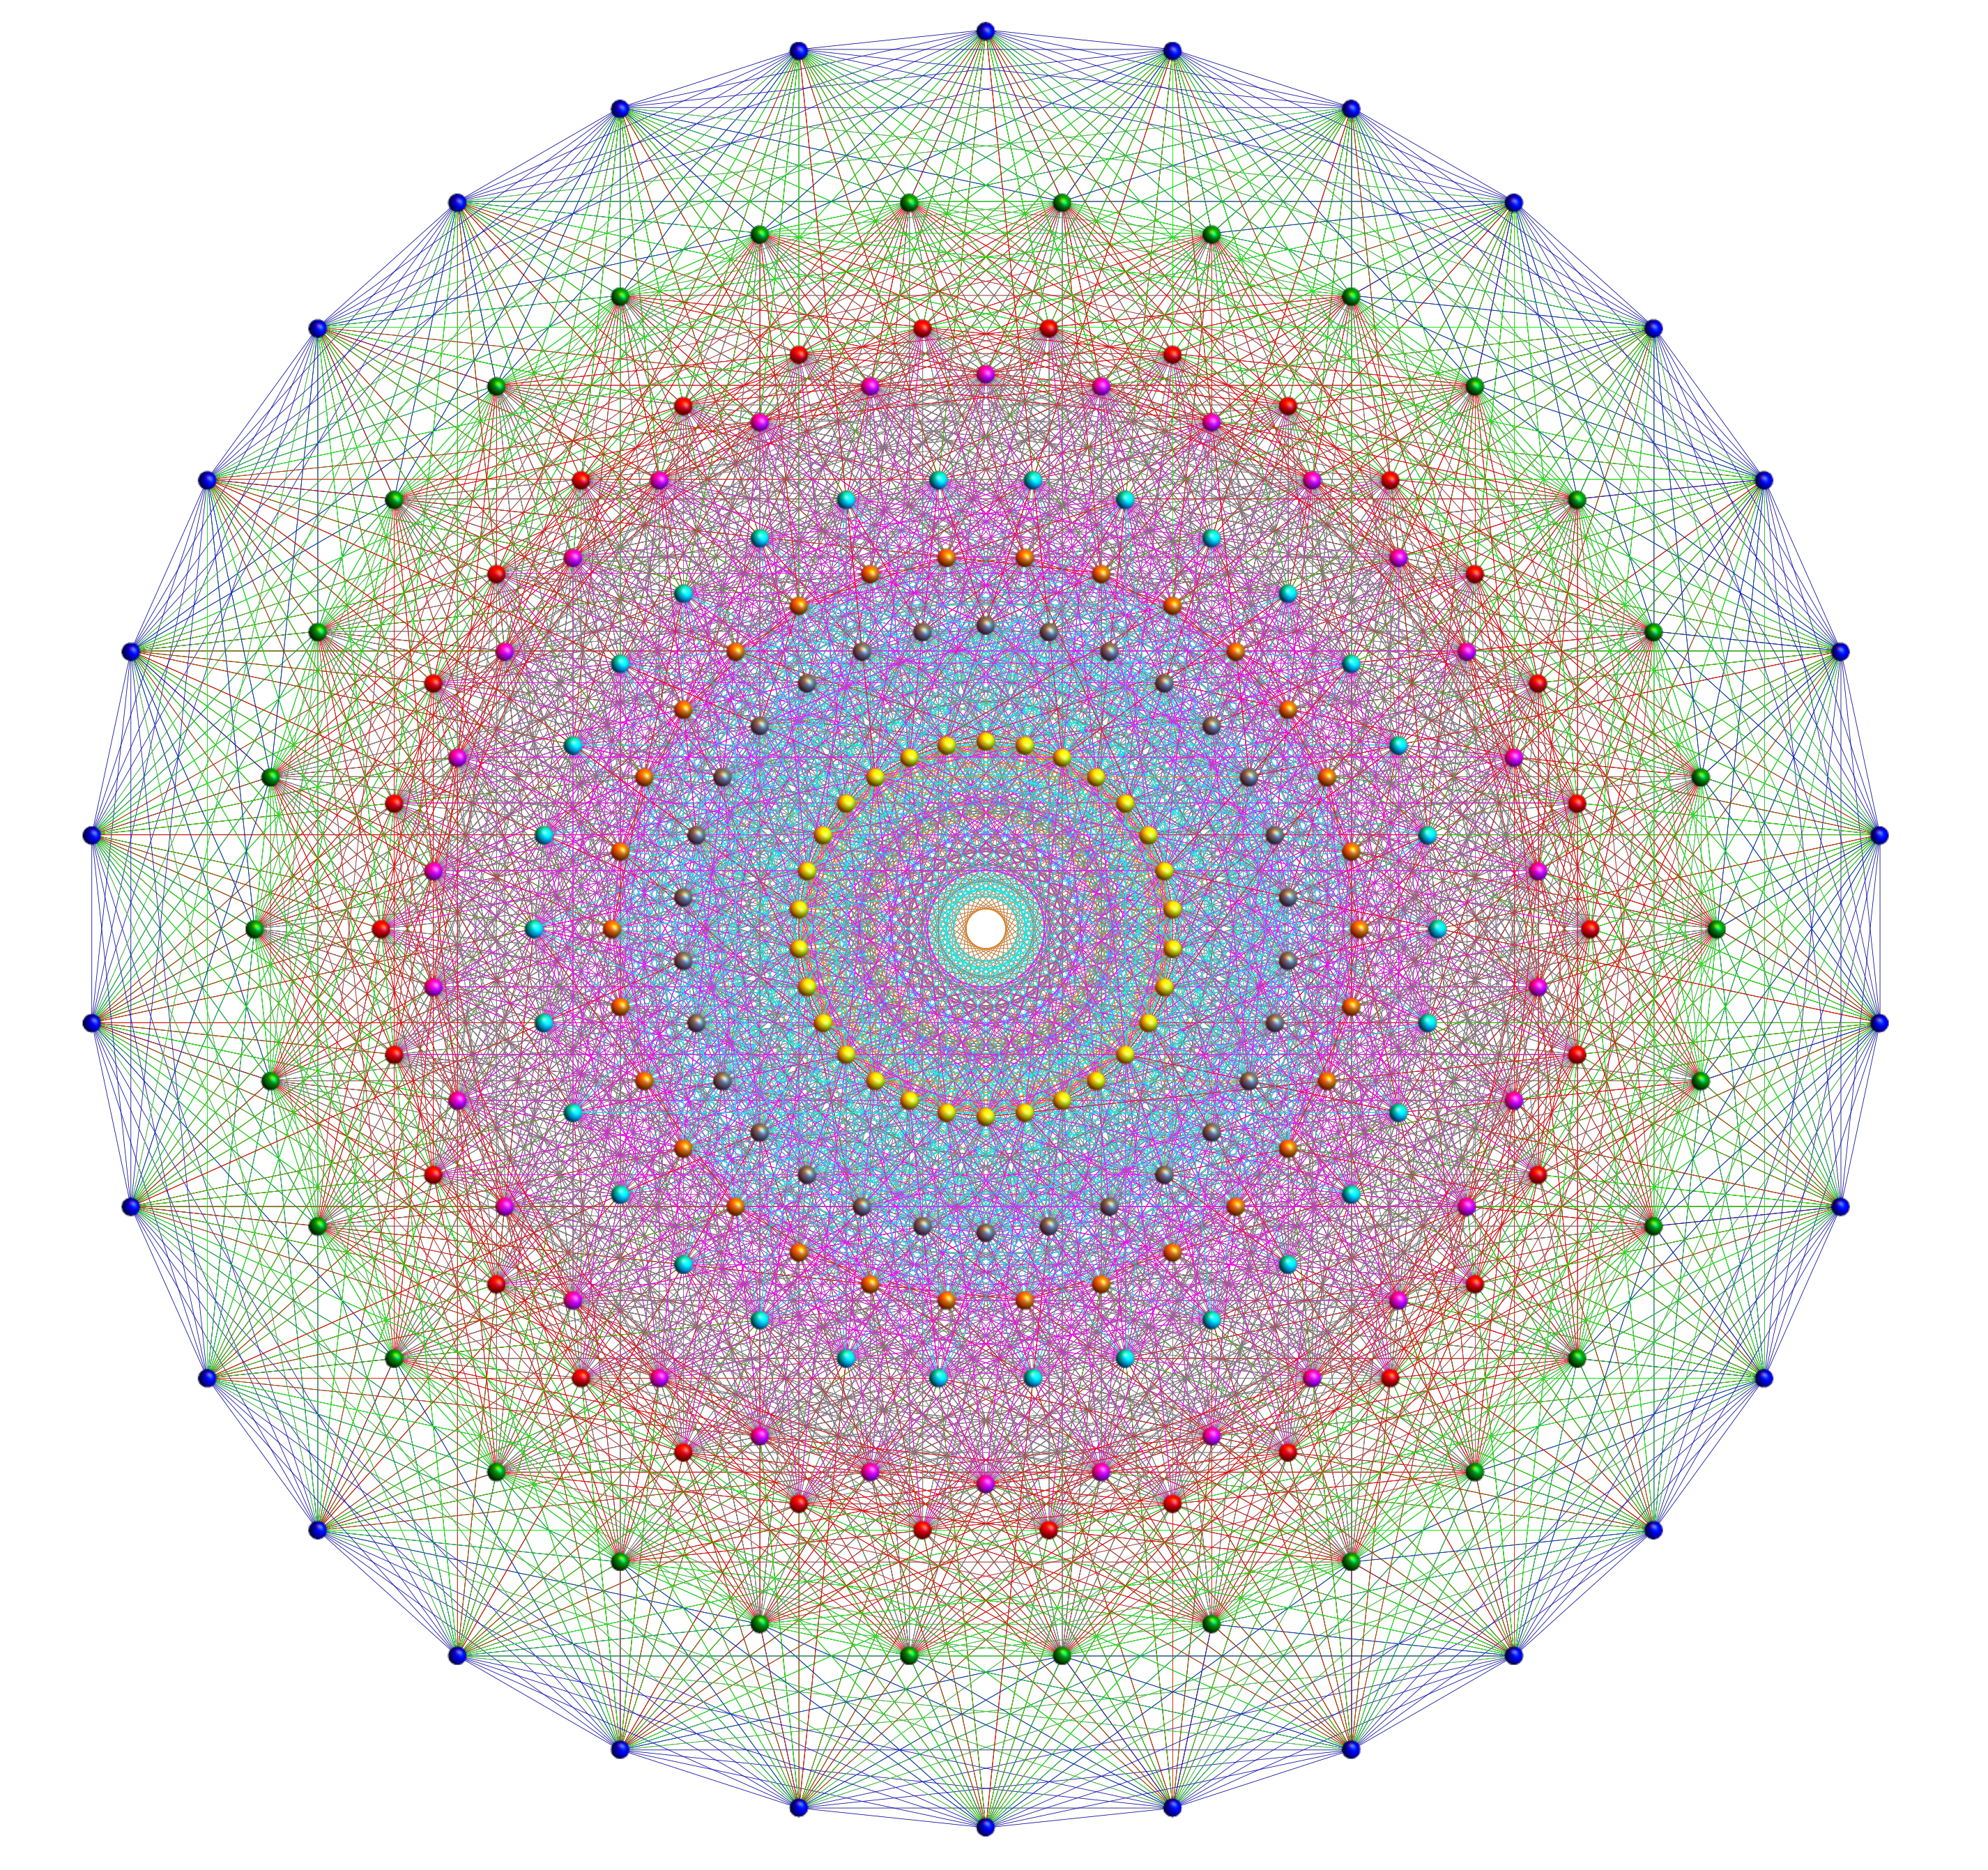
\includegraphics[width=.6\columnwidth]{front.jpg}
\end{figure}

\newpage
\pagestyle{plain}
\tableofcontents 
\newpage
\pagestyle{fancy}
\section{Teoria delle curve}
\subsection{Introduzione}
\begin{definizione}
	[Curva parametrizzata]
	Una \textit{curva paramtrizzata} \`e un'applicazione $\alpha  : I\subset \mathbb{R} \to \mathbb{R}^3$ di classe $C^\infty(I)$, con $I$ intervallo aperto.
	Data $t\in I$, si pu\`o scrivere in componenti come
	\[
	\alpha (t) = (x(t),y(t),z(t))
	\] 
	con $x,y,z:I\to \mathbb{R}$ tutte di classe $C^\infty(I)$.
\end{definizione}
\begin{osservazione}
La necessit\`a di definire la curva su un aperto, o quantomeno di poter estendere l'intervallo di definizione ad un aperto, deriva dal fatto che, in questo modo, si pu\`o effettivamente parlare di derivata piena anche per gli estremi, potendo trovare, infatti, un aperto che contiene interamente i punti di frontiera dell'intervallo di definizione.
Se non si avesse questa possibilit\`a, nel caso di $\alpha :[a,b] \subset \mathbb{R}\to \mathbb{R}^3$, per esempio, non si potrebbe calcolare la derivata tradizionale in $a$, o $b$, perch\'e si potrebbe solamente calcolare il limite destro o sinistro.
\end{osservazione}
\noindent Si nota che, nel caso in cui $I$ non fosse aperto, si estende l'intervallo di definizione ad $A \supset I$ aperto.

Si parla di \textit{traccia} della curva in riferimento all'immagine che genera dell'intero intervallo: $\operatorname{Tr} \alpha  = \alpha (I)$.
La traccia rappresenta l'unione di ciascun punto di $\alpha (t) \in \mathbb{R}^3, \ \forall t \in I$.
Per \textit{velocit\`a} della curva, invece, si intende la grandezza\footnote{Questa \`e ben definita perch\'e si sta operando in uno spazio vettoriale, con $\alpha (t+h) - \alpha (t)$ giustificata dall'operazione di somma dello spazio e divisione per $h$ data dalla moltiplicazione per uno scalare.}
\begin{equation}
	\alpha '(t) = \lim_{h \to 0} \frac{\alpha (t + h) - \alpha (t)}{h} = \big(x'(t),y'(t),z'(t)\big)
\end{equation}
In realt\`a, questo rappresenta il \textit{vettore velocit\`a}, mentre la velocit\`a vera e propria \`e data dalla sua norma $\left\lVert \alpha' (t) \right\rVert $.
\begin{esempio}
	[Retta parametrizzata]
	Siano $P,Q \in \mathbb{R}^3$, con $P\neq Q$, due punti dello spazio; si definisce, allora, \textit{retta parametrizzata} la curva 
	\[
		\alpha :
		\begin{array}
			{c c c}
			[0,1] &\longrightarrow & \mathbb{R}\\
			t &\longmapsto & P + t(Q-P) = P+t \overrightarrow{PQ}
		\end{array}
	\] 
La sua traccia \`e la retta affine passante per $P$ e $Q$, e ha vettore velocit\`a $\alpha '(t) = \overrightarrow{PQ}$, da cui $\left\lVert \alpha '(t) \right\rVert = \lVert \overrightarrow{PQ} \rVert$, che \`e costante.
\end{esempio}
\begin{esempio}
	[Circonferenza parametrizzata]
Dato $a\in \mathbb{R}$, con $a > 0$, si definisce \textit{circonferenza parametrizzata} come 
\[
\alpha:
	\begin{array}
		{c c c}
		[0,2\pi] &\longrightarrow & \mathbb{R}^3\\
		t &\longmapsto & (a \cos t, a \sin t , 0)
	\end{array}
\] 
il cui vettore velocit\`a \`e dato da $\alpha '(t) = (-a\sin t, a \cos t, 0)$, che non risulta costante, mentre la sua velocit\`a $\left\lVert \alpha ' \right\rVert = a >0$ s\`i.
La traccia corrisponde ad una circonferenza nel piano $z=0$, di centro l'origine e raggio $a$.
\end{esempio}
\subsection{Riparametrizzazione di una curva}
Sia $\alpha : [a,b]\to\mathbb{R}^3$ una curva parametrizzata; una sua \textit{riparametrizzazione} \`e data dalla coppia di mappe $h:[a,b]\to [c,d] \subseteq \mathbb{R}$ e $\beta : [c,d]\to \mathbb{R}^3$ tali che il diagramma
\[
\begin{tikzcd}
	\left[ a,b \right]  & & \mathbb{R}^3\\
	\\
	\left[ c,d \right] 
	\arrow[from=1-1, to=1-3, "\displaystyle \alpha "]
	\arrow[from=1-1,to=3-1,"\displaystyle h"']
	\arrow[from=3-1,to=1-3,"\displaystyle \beta"']
\end{tikzcd}
\] 
commuta, quindi si ha $\beta (h(t)) = \alpha (t)$. 
Perch\'e questo sia verificato, si assume che $h \in C^\infty([a,b])$ e $h'(t) \neq 0, \ \forall t \in [a,b]$; in questo modo, $\exists h^{-1}$ di classe $C^\infty$ tale che $\beta = \alpha \circ h^{-1}$, quindi anche $\beta $ risulta liscia ed \`e verificata la relazione $(\beta \circ h)(t) = \alpha (t)$, con $\operatorname{Tr} \alpha =\operatorname{Tr} \beta $.

Ora si definisce la lunghezza di una curva; se ne giustifica la definizione tramite il seguente ragionamento.
Sia dato $[a,b] \subset \mathbb{R}$ un intervallo e sia $P \in \mathcal{P} ([a,b])$ una sua partizione, tale che $a = t_0 < t_1 < \ldots<t_{k-1} <t_k = b$; allora la lunghezza di una curva $\alpha  : [a,b] \to \mathbb{R}^3$ approssimata a tale partizione \`e data da:
\begin{equation}
	L(\alpha , P) = \sum_{i=0}^{k-1} \left\lVert \alpha (t_{i+1}) - \alpha (t_i) \right\rVert 
\end{equation}
Si nota, dunque, che la lunghezza effettiva della curva coincide con
\begin{equation}
	\sup_{P \in \mathcal{P}([a,b]) } L(\alpha ,P) = \int_{a} ^b \left\lVert \alpha' (u) \right\rVert du
\end{equation}
\begin{definizione}
	[Lunghezza d'arco]
	Sia $\alpha  : [a,b] \subset \mathbb{R}\to \mathbb{R}^3$ una curva; si definisce \textit{lunghezza d'arco} la funzione
	\[
	s :
	\begin{array}
		{c c c}
		[a,b] & \longrightarrow &\mathbb{R}\\
		t & \longmapsto &\displaystyle  \int_{a} ^t \left\lVert \alpha '(u) \right\rVert du
	\end{array}
	\] 
	La lunghezza dell'intera curva $\alpha $ \`e data da $L(\alpha ) = s(b)$.
\end{definizione}
\begin{osservazione}
Si nota che per $\alpha : [0,+\infty) \to \mathbb{R}^3$, con $\alpha  (t) = \big(a \cos t, a \sin t, 0\big)$, valendo $\left\lVert \alpha '(t) \right\rVert = a$, si ha:
\[
s(t) = a \int_{0} ^t du = ta \implies s (2\pi) = 2\pi a
\] 
\end{osservazione}
\noindent Vale la pena chiedersi se $L(\alpha )$ sia indipendente dalla sua parametrizzazione, cio\`e se $L(\alpha ) = L(\beta )$, se $\beta $ \`e una riparametrizzazione di $\alpha $; questo si vede facilmente per conto diretto.
\begin{proof}
	Se $\alpha (t) = \beta (h(t))$, allora $\alpha '(t) = \beta '(h(t)) h'(t)$, quindi
	\[
	L(\alpha ) = \int_{a} ^b \left\lVert \alpha '(t) \right\rVert dt = \int_{a} ^b \lvert h'(t) \rvert \left\lVert \beta '(h(t)) \right\rVert dt
	\] 
	Ora si distinguono due casi: essendo $h'(t)\neq 0, \ \forall t$, si pu\`o avere o $h'(t) <0$, o $h'(t) > 0$. 
	Nel primo caso, si ha $h'(t) < 0$, quindi $\lvert h'(t) \rvert = - h'(t)$, con $h(a) = d$ e $h(b) = c$; nel secondo caso, $\lvert h'(t) \rvert =h'(t)$, con $h(a) = c$ e $h(b) = d$.
	Si trova, per $s = h(t)$, rispettivamente:
	\[
	\begin{cases}
		\displaystyle -\int_{d} ^c h'(t) \left\lVert \beta '(h(t))  \right\rVert dt = \int_{c} ^d \left\lVert \beta '(s) \right\rVert ds = L(\beta )\\
		\\
		\displaystyle \int_{c} ^d h'(t) \left\lVert \beta '(h(t)) \right\rVert dt = \int_{c} ^d \left\lVert \beta '(s) \right\rVert ds = L(\beta )
	\end{cases}
	\] 
In entrambi i casi, dunque, si ottiene $L(\alpha ) = L(\beta )$.	
\end{proof}
\noindent Ora si introduce una particolare riparametrizzazione, talvolta nota col nome di \textit{riparametrizzazione canonica}, o \textit{naturale}; per poterla definire, \`e necessario che $\alpha $ soddisfi la seguente condizione.
\begin{definizione}
	[Curva regolare]
	Una curva parametrizzata $\alpha : I \subset \mathbb{R} \to \mathbb{R}^3$ \`e detta \textit{regolare} se $\alpha '(t) \neq 0, \ \forall t \in I$.
\end{definizione}
\noindent Si considera, quindi, una curva regolare $\alpha :[a,b] \to \mathbb{R}^3$; visto che $s(t) = \int_{a} ^t \left\lVert \alpha '(u) \right\rVert du$, allora $s'(t) = \left\lVert \alpha '(t) \right\rVert >0$.
Si pu\`o pensare alla lunghezza d'arco come $s : [a,b] \to [0, L(\alpha )]$, che, essendo monotona perch\'e si \`e appena osservato che $s'(t) > 0$, allora ha anche inversa $t : [0,L(\alpha )]\to [a,b]$.
\`E, quindi, possibile definire la funzione 
\begin{equation}
	\beta = \alpha \circ t : [0,L(\alpha )]\to \mathbb{R}^3
\end{equation}
tale che $\operatorname{Tr} (\beta )=\operatorname{Tr} (\alpha ) $ e $\beta (s) = \alpha (t(s))$, per cui
\[
\beta '(s) = \alpha '(t(s)) t'(s) = \frac{\alpha '(t(s))}{s'(t(s))} = \frac{\alpha '(t(s))}{\left\lVert \alpha '(t) \right\rVert }
\] 
per cui $\left\lVert \beta '(s) \right\rVert =1$.
\begin{definizione}
	[Curva p.l.a.]
	Se $\alpha :I\to\mathbb{R}^3$ \`e una curva tale che $\left\lVert \alpha '(t)\right\rVert = 1 , \ \forall t \in I$, allora si dice che \`e \textit{parametrizzata tramite lunghezza d'arco}, o pla.
\end{definizione}
\begin{osservazione}
In base a quanto detto prima, ogni curva regolare \`e \textit{riparametrizzabile tramite lunghezza d'arco}.
\end{osservazione}
\begin{osservazione}
	[Non unicit\`a della versione pla]
	Data una curva regolare $\alpha  : I \to \mathbb{R}^3$, la riparametrizzazione tramite lunghezza d'arco non \`e univoca ma dipende dall'estremo inferiore di integrazione della lunghezza d'arco $s(t)$; se, infatti, $a,b \in I$ con $a < b$:
	\[
	s_a (t) = \int_{a} ^t \left\lVert \alpha '(u) \right\rVert du \hspace{1cm}s_b (t) \int_{b} ^t \left\lVert \alpha '(u) \right\rVert du
	\] 
	Le due, per\`o, differiscono solo per una costante perch\'e
	\[
	s_a(t) = \int_{a} ^b \left\lVert \alpha '(u) \right\rVert du + \int_{b} ^t \left\lVert \alpha '(u) \right\rVert du = \text{cost.} + s_b(t)
	\] 
	Questa differenza per una costante non influir\`a sulla trattazione del riferimento di Frenet perch\'e si lavora con derivate e la costante sparisce.
\end{osservazione}
\begin{esempio}
	[Elica]
Sia $a > 0$; allora la mappa
\[
\varphi :
\begin{array}
	{c c c}
	\mathbb{R}^2 & \longrightarrow & \mathbb{R}^3\\
	(u,z) &\longmapsto & (a \cos u , a \sin u , z)
\end{array}
\] 
definisce un cilindro di raggio $a$ attorno all'asse $z$.
Preso $b > 0$ e presi i punti $\left\{ (t,bt) \right\} _{t \in \mathbb{R}} $, relativi ad una retta passante per l'origine, aperto, si pu\`o definire la curva 
\[
\alpha (t) = \varphi (t,bt) = (a \cos t , a \sin t , bt)
\] 
che descrive un'\textit{elica destrorsa}, visto che si \`e preso $b>0$\footnote{Fosse stato $b<0$, sarebbe stata un'\textit{elica sinistrorsa}.}, di raggio $a$ e passo $b$.
Si nota che
\[
\alpha '(t) = (-a \sin t, a \cos t , b) \implies \left\lVert \alpha '(t) \right\rVert =\sqrt{a^2 + b^2} > 0, \ \forall t \in \mathbb{R}
\] 
da cui $\alpha $ \`e regolare. 
Restringendola a $[0,+\infty)$, cio\`e considerando $\alpha : [0,+\infty) \to \mathbb{R}^{3} $, si ha:
\[
	s(t) = \int_{0} ^t \sqrt{a^2 + b^2 }  du = t(s) \sqrt{a^2 + b^2} \implies t(s) = \frac{s}{\sqrt{a^2 +b^2}}
\] 
quindi:
\[
\begin{split}
		 \beta (s) &= \alpha (t(s)) = \alpha  \left(\frac{s}{\sqrt{a^2 + b^2} }\right) \\
	&= \left(a \cos \left(\frac{s}{\sqrt{a^2+b^2} }\right) , a\sin \left(\frac{s}{\sqrt{a^2 + b^2} }\right),\frac{bs}{\sqrt{a^2 + b^2} } \right)
	\end{split} 
\] 
con $\beta $ pla e, conseguentemente, $\beta (\mathbb{R}) = \operatorname{Tr} (\beta ) = \operatorname{Tr} (\alpha ) = \alpha (\mathbb{R})$.
\end{esempio}
\begin{esempio}
	[Ellisse]
	Siano $a,b \in \mathbb{R}\setminus\left\{ 0 \right\} $ e sia 
	\[
	\mathcal{E} _{a,b} = \left\{ (x,y,0) \in \mathbb{R}^3  \ \bigg\lvert \ \frac{x^2}{a^2} + \frac{y^2}{b^2} = 1\right\} \subset \mathbb{R}^3
	\] 
	Si vuole definire una curva $\alpha $ tale che $\operatorname{Tr} \alpha = \mathcal{E} _{a,b} $
\end{esempio}
	\begin{svolgimento}
		Si nota che $(x /  a , y / b) \in S^1$, cio\`e
	\[
	\frac{x}{a} = \cos t \hspace{1cm}\frac{y}{b} = \sin t
	\] 
	con $S^1$ circonferenza unitaria e $t\in [0,2\pi)$.
	Sia, allora
	\[
\alpha :
	\begin{array}
		{c c c}
		[0,2\pi) &\longrightarrow & \mathbb{R}^3\\
		t & \longmapsto & (a \cos t , b \sin t, 0)
	\end{array}
	\] 
 e si vede che $\operatorname{Tr} \alpha  = \mathcal{E} _{a,b} $.

	\end{svolgimento}
\begin{esempio}
Sia 
\[
\mathcal{C}  = \left\{ (x,y,0) \in \mathbb{R}^3  \mid y^2 = x^3 \right\}  \subset \mathbb{R}^3
\] 
Si vuole costruire $\alpha $ tale che $\operatorname{Tr}\alpha  = \mathcal{C} $.
\end{esempio}
\begin{svolgimento}
	Se si considera la secante $y = tx$, allora $t^2 x^2 = x^3$, ossia $x= t^2$ e $y = t^3$.
	Ne segue che la curva che soddisfa la richiesta \`e $\alpha (t) = (t^2 , t^3,0)$.
\end{svolgimento}
\begin{esempio}
Sia 
\[
\mathcal{C}  = \left\{ (x,y,0)  \mid y^2 = x^3 + x^2 \right\} \subset \mathbb{R}^3
\] 
Si vuole costruire una curva $\alpha $ tale che $\operatorname{Tr} \alpha  = \mathcal{C} $.
\end{esempio}
\begin{svolgimento}
	Si considera, come prima, $y=tx $, da cui $x^3 + x^2(1-t^2) = 0$, e si vede che $x = t^2 - 1$ e $y=t^3 -t$, quindi $\alpha (t) = (t^2 - 1, t^3-t,0)$.
\end{svolgimento}
\noindent Per quanto in linea teorica se $\alpha $ \`e una curva regolare, allora si pu\`o riparametrizzare tramite lunghezza d'arco, questo non \`e praticamente fattibile in ogni singolo caso; se, per esempio, si considera $\alpha (t) = (t,t^2,t^3)$, si ha $\alpha '(t) = (1,2t,3t^2)$, che, dunque, \`e regolare, ma data
\[
s(t) = \int_{0} ^t \sqrt{1 + 4u^2 + 9u^4} du
\] 
non si \`e in grado di trovare un'espressione per $t(s)$ perch\'e la primitiva di $s$ non \`e scrivibile in termini di funzioni elementari.
\subsection{Riferimento ed equazioni di Frenet}
\begin{definizione}
	[Versore tangente]
	Data una curva riparametrizzabile $\alpha :I \to \mathbb{R}^3$ e la sua riparametrizzazione tramite lunghezza d'arco $\beta (s)$, si definisce il \textit{versore tangente} ad $\alpha $ come $T(s) = \beta '(s)$.
\end{definizione}
\begin{definizione}
	[Curvatura]
	Data una curva pla $\beta :I\to \mathbb{R}^3$ e il suo versore tangente $T(s)$, allora se ne definisce la \textit{curvatura} come
	\[
	k (s) = \left\lVert T'(s) \right\rVert 
	\] 
\end{definizione}
\noindent Ora si ricavano il riferimento di Frenet e le equazioni di Frenet.
Per poter definire il riferimento di Frenet e ricavare, conseguentemente, le equazioni di Frenet, \`e necessario imporre ulteriori condizioni sulle curve in esame; la condizione operativa necessaria \`e la seguente.
\begin{definizione}
	[Curva di Frenet]
	Una curva regolare $\alpha:[a,b]\to\mathbb{R}^3 $ \`e detta \textit{di Frenet} se la sua pla $\beta = \alpha  \circ t:[0,L(\alpha )]\to \mathbb{R}^3$ \`e tale che $k(s) >0, \ \forall s \in [0,L(\alpha )]$.
\end{definizione}
\begin{lemma}\label{lemdif}
	Se $f, g : I \to \mathbb{R}^{3} $ sono due mappe, allora 
	\[
	\left(f(t)\cdot g(t)\right) ' = f'(t) \cdot g(t) + f(t) \cdot g'(t)
	\] 
\end{lemma}
	\begin{proof}
		Si ha
		\[
		f(t) \cdot g(t) = \sum_{i=1}^{3} f_i(t) g_i(t)
		\] 
	quindi
	\[
	\left(f(t)\cdot g(t)\right) ' = \sum_{i=1}^{3} \left[ f_i'(t)g_i(t) + f_i(t) g_i'(t) \right] 
	\] 
	\end{proof}
\noindent Data $\alpha : I \to \mathbb{R}^3$ una curva di Frenet e $T(s) = \beta '(s)	$ il suo versore normale, con $\beta $ versione pla di $\alpha $, si nota che $T'(s)$ non \`e, in generale un versore e 
\[
1 = \left\lVert T(s) \right\rVert ^2 = T(s) \cdot T(s) \implies \left[ T(s) \cdot T(s) \right] ' = 2T'(s) \cdot T(s) = 0 \implies T'(s) \perp T(s) 
\] 
Avendo assunto $\alpha $ di Frenet, significa che $k_\alpha  (s) \neq 0$, quindi $T'(s)$ \`e normalizzabile e si ottiene un versore ortogonale a $T(s)$.
Usando questo versore e $T(s)$, tramite il prodotto vettore, se ne pu\`o definire un terzo; allora si ha la seguente definizione.
\begin{definizione}
	[Versori normale e binormale]
	Dato $T(s)$ versore tangente di una curva di Frenet $\alpha : I \to \mathbb{R}^3$, si definiscono $N(s) = T'(s) / \left\lVert T'(s) \right\rVert $ \textit{versore normale principale} e $B(s) = T(s) \times N(s)$ \textit{versore binormale}.
\end{definizione}
\noindent Evidentemente, si ha $\left\lVert N(s) \right\rVert =\left\lVert B(s) \right\rVert  = 1 $ e $T(s) \cdot N(s) = T(s) \cdot B(s) = N(s) \cdot B(s) =  0 $.
Ne segue che $\big(T(s),N(s),B(s)\big), \ \forall s \in I$ forma una base ortonormale di $\mathbb{R}^3$, nota col nome di \textbf{riferimento di Frenet}.
Per definizione di $N(s)$, si ottiene la \textbf{I equazione di Frenet}:
\begin{boxenv}[]
\begin{equation}
	T'(s) = k(s) N(s)
\end{equation}
\end{boxenv}
\noindent Si nota che, essendo un versore, si ha $N(s) \cdot N(s) = 1$, quindi $N'(s) \cdot N(s) = 0$ (per lo stesso ragionamento fatto per $T(s)$), dunque $N'(s) \in \langle T(s) , B(s) \rangle$; inoltre, essendo $T(s)\cdot N(s) = 0$, si ha 
\[
	T'(s) \cdot N(s) +T(s)\cdot  N'(s)=k(s) \underbracket{N(s) \cdot N(s)}_{=1}  +T(s)\cdot  N'(s) = 0 
\] 
perci\`o si trova $ \tau (s)$ tale per cui 
\begin{boxenv}[]
\begin{equation}
	N'(s) = -k(s)  T(s) + \tau (s)  B(s)
\end{equation}
\end{boxenv}
\noindent Questa \`e nota come \textbf{II equazione di Frenet}.
\begin{definizione}
	[Torsione]
	Data una curva regolare $\alpha :I\to\mathbb{R}^3$ e $\beta $ la sua pla, si definisce $\tau (s)$ come la \textit{torsione} di $\beta $ nel punto $s$.
\end{definizione}
\noindent Ripetendo lo stesso ragionamento, si ha $B(s) \cdot B(s) = 1 \Rightarrow B'(s) \cdot B(s) = 0$, da cui $B'(s) \in \langle T(s),N(s) \rangle$ e, essendo $N(s) \cdot B(s) = 0$, dalla derivata di $T(s) \cdot B(s) = 0$, si ha
\[
	T'(s) \cdot B(s) + T(s) \cdot B'(s) = k(s) \underbracket{N(s) \cdot B(s)}_{=0}  + T(s) \cdot B'(s) = 0
\] 
quindi $B'(s) \in \langle N(s) \rangle$.
Usando $T(s) \cdot B(s) = 0 $ e derivando $N(s) \cdot B(s) = 0$, si ottiene
\[
	\begin{split}
		N'(s) \cdot B(s) + N(s) \cdot B'(s) &= (- k(s) T(s) + \tau (s) B(s) )\cdot B(s) + N(s) \cdot B'(s) \\
		&= \tau (s) \underbracket{B(s)\cdot B(s)}_{=1}  + N(s)\cdot B'(s) = 0 
	\end{split}
\] 
cio\`e
\begin{boxenv}[]
\begin{equation}
	B'(s) = - \tau (s) N(s)
\end{equation}
\end{boxenv}
\noindent che \`e nota come \textbf{III equazione di Frenet}.
Ricapitolando, le equazioni di Frenet stabiliscono delle relazioni tra le derivate dei versori ortonormali del riferimento di Frenet e i versori stessi e sono:
\begin{boxenv}[]
\begin{equation}
	\begin{cases}
		T'(s) = k(s) N(s)\\
		N'(s) = - k(s) T(s) + \tau (s) B(s)\\
		B'(s)=-\tau (s) N(s)
	\end{cases}
\end{equation}
\end{boxenv}
\noindent Ora si applicano i concetti visti alle curve studiate nella sezione precedente.
\begin{esempio}
	Sia $\alpha (t) = P + t \overrightarrow{PQ}$ una curva parametrizzata (con $P,Q \in \mathbb{R}^3$ e $P\neq Q$). 
	Si ha $\alpha '(t) = \overrightarrow{PQ}$, quindi la curva \`e regolare, quindi se ne pu\`o trovare una pla:
	\[
		s(t) = \int_{a} ^t \lVert \overrightarrow{PQ} \rVert du= t \lVert \overrightarrow{PQ} \rVert \implies t = \frac{s}{\lVert \overrightarrow{PQ} \rVert }
	\] 
	quindi si ha $\beta (s) = P + s \frac{\overrightarrow{PQ}}{\lVert \overrightarrow{PQ} \rVert }$. 
	Allora il versore tangente \`e dato da 
	\[
	T(s) = \beta '(s) = \frac{\overrightarrow{PQ}}{\lVert \overrightarrow{PQ} \rVert } \implies T'(s) = 0 
	\] 
	perci\`o $k(s) = 0$ e, quindi, $\alpha $ non \`e una curva di Frenet perch\'e non ha curvatura positiva.
\end{esempio}
\begin{esempio}
Per $a>0$, sia $\alpha (t) = (a \cos t, a \sin t, 0)$ una circonferenza parametrizzata di raggio $a$.
Evidentemente, si pu\`o vedere come un caso particolare di elica parametrizzata per $b=0$, quindi si pu\`o fare uso del risultato trovato in precedenza:
\[
	\begin{split}
		&\beta (s) = \left(a \cos \left(\frac{s}{a}\right) , a\sin \left(\frac{s}{a}\right),0 \right)\implies T(s) = \left(- \sin \frac{s}{a}, \cos \frac{s}{a},0 \right) \\
		&\Rightarrow T'(s) = \underbracket{\frac{1}{a}}_{k(s)}  \underbracket{\left(-\cos \frac{s}{a},- \sin \frac{s}{a},0\right) }_{N(s)} 
	\end{split}
\] 
Si conclude che $N(s)\perp z$ e punta proprio verso $z$; inoltre, la circonferenza parametrizzata \`e una curva di Frenet perch\'e ha curvatura positiva, essendo $1 / a > 0 $ perch\'e $a > 0 $ per assunzione.
Infine:
\[
	\begin{split}
		&B(s) = \begin{pmatrix} -\sin s / a \\ \cos s / a \\ 0  \end{pmatrix} \times \begin{pmatrix} - \cos s / a\\ - \sin s / a \\ 0  \end{pmatrix} = \begin{pmatrix} 0 \\0 \\ 1 \end{pmatrix} \\
		&\Rightarrow -\tau (s) N(s) = B'(s) = 0 \implies \tau (s) = 0 
	\end{split}
\] 
\end{esempio}
\begin{esempio}
Si considera l'elica parametrizzata $\alpha = (a\cos t , a \sin t, bt)$, con raggio $a\in \mathbb{R}^{>0} $ e passo $b \in \mathbb{R}$.
La sua pla \`e gi\`a stata ricava; dato $c = \sqrt{a^2 + b^2} $, si ottiene:
\[
	\beta (s)= \left(a \cos \left(\frac{s}{\sqrt{c} }\right) , a\sin \left(\frac{s}{\sqrt{c} }\right),\frac{b}{\sqrt{c} } s\right)
\] 
da cui
\[
	T(s) = \frac{1}{c}\left(-a \sin \frac{s}{c}, a \cos \frac{s}{c}, b\right) \implies T'(s) = \underbracket{\frac{a}{c^2}}_{k(s)} \underbracket{\left(-\cos \frac{s}{c},- \sin \frac{s}{c},0\right) }_{N(s)} 
\] 
quindi, come nel caso della circonferenza, $N(s)\perp z$ e punta verso di esso.
Si ha:
\[
B(s) = \frac{1}{c} \begin{pmatrix} - a \sin s / c\\ a \cos s / c\\ b  \end{pmatrix} \times \begin{pmatrix} - \cos s / c \\ - \sin s / c \\ 0  \end{pmatrix} = \frac{1}{c} \begin{pmatrix} b \sin s / c \\ - b \cos  s / c \\ a  \end{pmatrix} 
\] 
Inoltre:
\[
	N'(s) = - k(s) T(s) +\tau (s) B(s) \implies \tau (s) = N'(s) \cdot B(s) =  \frac{b}{c^2}
\] 
Da questo, si vede che
\begin{itemize}
	\item se $b>0$, allora l'elica \`e destrorsa e $\tau (s) >0$,
	\item se $b<0$, allora l'elica \`e sinistrorsa e $\tau (s) < 0 $,
	\item se $b=0$, si ha una circonferenza e $\tau (s) = 0 $, con $k(s) = 1 / a$.
\end{itemize}
Fissando $a$, si nota che, per $b \to \pm \infty$, si ha $\tau (s) \to 0$ e $k(s) = a / (a^2 + b^2) \to 0 $.
\end{esempio}
\begin{prop}
	Sia $\alpha  : I \to \mathbb{R}^3$ una curva regolare; allora $k_\alpha = 0 \iff \alpha (I)$ \`e contenuta in una retta.
\end{prop}
	\begin{proof}
		Si divide la dimostrazione nelle due implicazioni.
		\begin{itemize}
			\item ($\Leftarrow$) Se $\alpha (I) \subseteq P+ \langle v \rangle$, per $v$ versore generico, si considera la sua versione pla $\alpha (I) = \beta (J) \subseteq P+\langle v \rangle$; allora $\beta = P + f(s) v$ e $\beta '=f'(s) v$, con $f'(s)=\pm 1$ perch\'e $\left\lVert \beta ' \right\rVert = 1$. 
				Ne segue che:
				\[
				T(s) = \beta '(s) = f'(s) v = \pm v \implies T'(s) = 0 \implies k_\alpha(s) = 0 
				\] 
			\item ($\Rightarrow $) Sia $\left\lVert T'(s) \right\rVert = k_\alpha (s) = 0 $, quindi $T(s) = \beta '(s) = v $, per qualche $v \in \mathbb{R}^3$.
				Allora si deve avere $\beta (s) =  \beta (0)+ s v \in \beta (0) +\langle v \rangle$.
		\end{itemize}
	\end{proof}
\begin{esercizio}
Sia $\beta :I \to \mathbb{R}^3$ una curva pla tale che
\[
\beta (I) \subseteq S_r^2(P) = \left\{ x \in \mathbb{R}^3 \ \big\lvert\ \left\lVert x- P \right\rVert = r\right\} 
\] 
Mostrare che $\beta  $ \`e di Frenet.
\end{esercizio}
\begin{svolgimento}
	Se $\beta (I) \subseteq S_r^2(P)$, allora $\left\lVert \beta (s) - P \right\rVert ^2 = r^2$; derivando due volte rispetto a $s$, si ottiene:
	\[
		\begin{split}
			&\frac{d }{d s}\left[  T(s) \cdot (\beta (s) - P )  \right] = 0 \implies T'(s) \cdot (\beta (s) - P) + T(s) \cdot T(s) = 0 \\
			&\Rightarrow T'(s) \cdot (\beta (s) - P) = -1 \implies k(s) \left[ N(s) \cdot (\beta (s) - P) \right] = - 1
		\end{split}
	\] 
	Quindi $k(s) \neq 0$ e, pertanto $\beta $ \`e di Frenet.
\end{svolgimento}
\begin{prop}
	Sia $\alpha  : I \to \mathbb{R}^3$ una curva di Frenet; allora $\tau _\alpha = 0 \iff \alpha (I)$ \`e contenuta in un piano.
\end{prop}
	\begin{proof}
		Si divide la dimostrazione nelle due implicazioni.
		\begin{itemize}
			\item ($\Rightarrow $) Si assume, senza perdita di generalit\`a, che $\alpha $ sia pla\footnote{Altrimenti, $\alpha $ ammette una versione pla perch\'e \`e una curva di Frenet.}.
				Allora 
				\[
				\tau _\alpha  = 0 \implies B'_\alpha (s) = - \tau _\alpha (s) N_\alpha (s) = 0 
				\] 
				quindi $B_\alpha $ \`e costante; sia $B_\alpha (s) = B_0$, per qualche $B_0\in \mathbb{R}^3$ tale che $\left\lVert B_0 \right\rVert =1$.
				Ne segue, allora, che
				\[
				T(s) \cdot B_0 = \alpha '(s) \cdot B_0\implies (\alpha (s) \cdot B_0)' = 0
				\] 
				quindi $\alpha (s)\cdot B_0 = c \in \mathbb{R}$, dunque $\alpha (I) \subseteq \left\{ x \in \mathbb{R}^3  \mid x\cdot B_0 = c \right\} $.
			\item ($\Leftarrow$) Sia $\alpha (I) \subseteq \left\{ x \in \mathbb{R}^3  \mid x\cdot B_0 =c  \right\} $, per qualche $B_0 \in \mathbb{R}^3$ tale che $\left\lVert B_0  \right\rVert  = 1$ e $c \in \mathbb{R}$; allora $\forall s, \ \alpha (s) \cdot B_0 = c$.
				Ne segue che
				\[
				T(s) \cdot B_0 = 0 \implies k(s) (N(s) \cdot B_0) = 0 \implies N(s) \cdot B_0 = 0
				\] 
				dove la seconda implicazione \`e giustificata dal fatto che $\alpha $ \`e di Frenet, quindi $k(s) > 0 $.
				Visto che $B_\alpha (s) = T(s) \times N(s)$, considerando (continuare \ldots).
		\end{itemize}
	\end{proof}
\begin{prop}
	Sia $\alpha : I \to \mathbb{R}^3$ una curva di Frenet; se $\tau _\alpha  = 0$, allora $k_\alpha $ \`e costante $\iff \alpha (I)$ \`e contenuta in una circonferenza.
\end{prop}
\begin{proof}
{\color{nred} Da scrivere\ldots}
\end{proof}
\begin{prop}
	Sia $\alpha : I \to \mathbb{R}^3$ una curva regolare; se $\alpha (I) \subseteq \mathbb{S}_R(P) = \left\{ x \in \mathbb{R}^3  \mid \left\lVert x - P \right\rVert = R \right\} $, allora $\alpha $ \`e di Frenet e $k_\alpha \ge 1 / R > 0$.
\end{prop}
\begin{proof}
	Sia $\beta $ la versione pla di $\alpha $. Assumendo che $\operatorname{Tr} (\beta ) \subseteq \mathbb{S}_R(P)$, si ha:
	\[
		(\beta (s) - P) \cdot (\beta (s) - P) = \left\lVert \beta (s) - P \right\rVert ^2 = R^2
	\] 
	Derivando questa relazione, si ha:
	\[
	\beta '(s) \cdot (\beta (s) - P) = 0
	\] 
	Derivando nuovamente:
	\[
		T'(s) \cdot (\beta (s)-P) + \underbracket{\beta '(s) \cdot \beta '(s)}_{=1}  = 0 
	\] 
	Passando alla norma, si vede che:
	\[
	1=\left\lVert T'(s) \cdot (\beta (s) - P) \right\rVert \le \left\lVert T'(s) \right\rVert \left\lVert \beta (s) - P \right\rVert = k_\alpha (s) R
\] 
	da cui $k_\alpha (s) \ge 1 / R > 0$, quindi $\alpha $ \`e di Frenet.
\end{proof}
\subsection{Riferimento di Frenet senza lunghezza d'arco}
Come accennato, la possibilit\`a di ottenere la versione pla di una curva regolare, anche se ammissibile in teoria, non sempre \`e concreta in pratica.

Sia, allora, $\alpha : I \to \mathbb{R}^3$ una curva regolare; per definzione
\[
	\beta (s(t))= \alpha (t) \implies \beta '(s(t)) s'(t) = \beta '(s(t)) \left\lVert \alpha '(t) \right\rVert = \alpha '(t)
\] 
da cui si ottiene la relazione
\begin{boxenv}[]
\[
	T(s(t)) = \frac{\alpha '(t)}{\left\lVert \alpha '(t) \right\rVert }
\] 
\end{boxenv}
\noindent Dalla relazione precedente, sostituendo $\beta '(s(t)) = T(s(t))$, si ottiene
\begin{equation}
	s'(t) T(s(t)) = \alpha '(t)
\end{equation}
e, derivando:
\begin{equation}\label{e1}
s'' (t) T(s(t)) + s'^2(t) T'(s(t)) = \alpha ''(t)
\end{equation}
A questo punto, si vede che, facendo il prodotto vettore $\alpha ' \times \alpha ''$, il termine $T' \times T' = 0$, quindi:
\begin{equation}\label{e2}
	\alpha ' \times \alpha '' = s'^3 T\times T'
\end{equation}
Si nota che, essendo $T ' \perp T $ e $\left\lVert T \right\rVert = 1$, si ha $\left\lVert T ' \times T \right\rVert = \left\lVert T' \right\rVert = k$, perci\`o
\begin{boxenv}[]
\[
k = \frac{\left\lVert \alpha '\times \alpha '' \right\rVert }{s'^3}= \frac{\left\lVert \alpha ' \times \alpha ''\right\rVert }{\left\lVert \alpha '\right\rVert ^3}
\] 
\end{boxenv}
\noindent Per continuare, si assume che $\alpha $ sia una curva di Frenet; allora, usando la I equazione di Frenet, si ottiene
\[
	s'^3 k \underbracket{T \times N }_{=B} = \alpha ' \times \alpha ''
\] 
da cui si ottiene
\begin{boxenv}[]
\[
B=\frac{\alpha '\times \alpha ''}{\left\lVert \alpha ' \right\rVert ^3 k} =\frac{\alpha ' \times \alpha ''}{\left\lVert \alpha ' \times \alpha '' \right\rVert }
\] 
\end{boxenv}
\noindent Da questo, si ricava 
\begin{boxenv}[]
\[
N = B \times T = \frac{\alpha ' \times \alpha '' \times \alpha '}{\left\lVert \alpha '\times \alpha '' \right\rVert \left\lVert \alpha ' \right\rVert }
\] 
\end{boxenv}
\noindent Infine, si calcola la torsione. 
Per farlo, si deriva la I equazione di Frenet:
\[
s'T'' = s'k'N + s'k N'  \implies T'' = k'N + kN'
\] 
dove $s' \neq 0$ perch\'e la curva \`e regolare e, quindi, si cancella.
Vista la III equazione di Frenet $B'  = -\tau N $, si ha $\tau  = - B' \cdot N$; in realt\`a, si nota che
\[
	0=(\underbracket{B\cdot N}_{=0} )'= B' \cdot N + B \cdot N'\implies B' \cdot N = - B\cdot N'
\] 
da cui $\tau  = B \cdot N'$.
Derivando l'equazione \ref{e1}:
\[
\alpha '''= T'' s'^3 + 3T's's'' + Ts''' 
\] 
Ora, visto che $T' \propto N$ e $T,N \perp B$, dal prodotto scalare per $B$ si ha:
\[
\alpha ''' \cdot B = s'^3T '' \cdot B = s'^3k N' \cdot B= s'^3 k \tau 
\] 
Ricordando l'espressione per $B$, si ha:
\begin{boxenv}[]
\[
\tau = \frac{\alpha ''' \cdot (\alpha ' \times \alpha '')}{\left\lVert \alpha ' \times \alpha '' \right\rVert ^2 } 
\] 
\end{boxenv}
\begin{osservazione}
L'esistenza di queste formule implica l'indipendenza di curvatura, torsione e intero riferimento di Frenet dalla scelta della lunghezza d'arco per la riparametrizzazione.
\end{osservazione}
\subsection{Teorema fondamentale della teoria delle curve}
Siano $\beta , \widetilde{\beta }:I\to \mathbb{R}^3$ due curve pla di Frenet, con $\widetilde{\beta }$ ottenuta tramite roto-traslazione di $\beta $, cio\`e
\[
\widetilde{\beta }(s) = A \beta (s) + b
\] 
con $A \in \mathrm{SO} (3)$ e $b \in \mathbb{R}^3$.
Quello che si vuole verificare ora \`e che le due curve abbiano uguali curvatura e torsione.
Per farlo, si nota che, essendo $A$ un operatore lineare, \`e anche continuo (visto che opera su uno spazio finito-dimensionale), dunque:
\[
\widetilde{T}(s) = A T(s)  \hspace{1cm} \widetilde{T}' (s) = T'(s) \implies \widetilde{k}(s) \widetilde{N}(s) = k(s) A N(s)
\] 
$\forall s \in I $.
Passando alle norme, visto che $A$ le preserva si ha $\left\lVert A N(s) \right\rVert = 1, \ \forall s \in I $, dunque $\widetilde{k}(s) = k(s), \ \forall s \in I$.

Per la torsione, invece, si ha:
\[
\widetilde{B}(s) = \widetilde{T}(s) \times \widetilde{N}(s) = (AT(s)) \times (AN(s)) = A\left[ T(s) \times N(s) \right] = A B(s)
\] 
Per passaggi analoghi a prima, si vede che 
\[
\widetilde{B}'(s) = A B'(s) \implies -\widetilde{\tau }(s) \widetilde{N}(s) = - \tau (s) A N(s)
\] 
da cui $\widetilde{\tau }(s) = \tau (s)$.
Ora ci si chiede il viceversa: date due curve con uguale curvatura e torsione, \`e vero che una \`e la versione roto-traslata dell'altra?
Per rispondere, si ha il seguente.
\begin{teorema}
	Se $\beta ,\widetilde{\beta }:I\to\mathbb{R}^3$ sono due pla di Frenet con $k(s) = \widetilde{k}(s)$ e $\tau (s)= \widetilde{\tau }(s)$, allora $\exists A \in \mathrm{SO} (3), \ \exists b \in \mathbb{R}^3$ tali che $\widetilde{\beta }(s) = A \beta (s) + b , \ \forall s \in I$.
\end{teorema}
\subsection{Esercizi}
\begin{esercizio}
Sia data la curva
\[
	\alpha :
\begin{array}
	{c c c}
	\mathbb{R}&\longrightarrow& \mathbb{R}^3\\
	t&\longmapsto &\left(\frac{1}{3}t^3, \sqrt{2} (t \sin t + \cos t), \frac{1}{2}(t + \sin t \cos t)\right) 
\end{array}
\] 
Rispondere ai seguenti punti.
\begin{enumerate}[(a).]
	\item Dimostrare che $\alpha $, ristretta ad un intorno dell'origine, \`e di Frenet.
	\item Calcolare la curvatura e il riferimento di Frenet in un intorno di $t=0$.
\end{enumerate}
\end{esercizio}
\begin{svolgimento} Per lo svolgimento, si user\`a la seguente definizione di lunghezza d'arco:
	\[
	s(t) := \int_{0} ^t \left\lVert \alpha '(u) \right\rVert du
	\] 
	Si divide lo svolgimento nei due punti.
	\begin{enumerate}[(a).]
		\item Essendo interessati ad un intorno dell'origine, per dire che $\alpha $ \`e di Frenet bisogna preliminarmente verificarne la regolarit\`a; allora si nota che
			\[
			\alpha ' = \left(t^2 , \sqrt{2} t \cos t, \cos^2 t\right) 
			\] 
			che \`e non-nulla in un intorno di $t=0$.  
			Ora, invece di procedere direttamente con i conti, che sono estremamente lunghi e complessi, si pu\`o notare che la condizione da mostrare \`e $T'(0) \neq 0$, per far vedere ce $\alpha $ \`e di Frenet in un intorno dell'origine.
			Per farlo, si pu\`o mostrare che $T \cdot T' \neq 0$ in $s(0)$ e si possono usare le relazioni
			\[
			\alpha ' (t) = s'(t) T(s(t)) \hspace{1cm}\alpha ''(t) =s''(t)T(s(t)) + s'^2 (t) T'(s(t))
			\] 
			Infatti
			\[
			\alpha ' \times \alpha '' = \left\lVert \alpha ' \right\rVert ^3 T \times T'
			\] 
			e $\alpha ''$ si calcola facilmente come
			\[
			\alpha ''(t)  =\left(2t , \sqrt{2} (\cos t - t \sin t),-2 \cos t \sin t\right) 
			\] 
			Quindi 
			\[
			\alpha '(0) \times  \alpha ''(0) = \begin{pmatrix} 0\\ 0 \\ 1  \end{pmatrix} \times \begin{pmatrix} 0 \\\sqrt{2} \\0 \end{pmatrix} = \begin{pmatrix} -\sqrt{2} \\ 0 \\ 0 \end{pmatrix} 
			\] 
		che permette di concludere direttamente che $T' \neq 0$ in un intorno di $t=0$.
	\item 	Si nota che, essendo 
		\[
		\left\lVert \alpha ' \right\rVert = \sqrt{t^4 + 2 t^2 \cos^2 t + \cos^4 t} = t^2 + \cos^2 t \Rightarrow \left\lVert \alpha '(0) \right\rVert = 1
		\] 
		allora, dalla norma di $\alpha '(0) \times \alpha ''(0)$, si ricava:
		\[
		\sqrt{2} = \underbracket{\left\lVert \alpha '(0) \right\rVert ^3}_{=1} k\implies k(0) = \sqrt{2} 
		\] 
		Dalla stessa relazione, si ricava anche $B$, inserendo la I equazione di Frenet:
		\[
		\begin{pmatrix} - \sqrt{2} \\0 \\0 \end{pmatrix} = T \times T' = k T \times N = k B \implies B(0) = \begin{pmatrix} -1 \\0 \\0  \end{pmatrix} 
		\] 
	Dai calcoli precedenti, si pu\`o ottenere il versore tangente in $t=0$:
	\[
	T(0) = \frac{\alpha '(0)}{\left\lVert \alpha '(0) \right\rVert } = \begin{pmatrix} 0 \\ 0 \\ 1 \end{pmatrix} 
	\] 
	Per finire, si ottiene il versore normale tramite prodotto vettore:
	\[
	N(0) = B(0) \times T(0) = \begin{pmatrix} -1 \\0 \\0 \end{pmatrix} \times \begin{pmatrix} 0\\0\\ 1 \end{pmatrix} = \begin{pmatrix} 0 \\ 1 \\0 \end{pmatrix} 
	\] 
	\end{enumerate}
\end{svolgimento}











\end{document}

